\documentclass[10pt, letterpaper]{article}
\usepackage{amssymb}
\usepackage[utf8]{inputenc}
\usepackage{amsmath}
\usepackage[spanish]{babel}
\usepackage{tikz}
\usepackage{graphicx}
\newcommand{\N}{\mathbb{N}}
\newcommand{\R}[1]{$\mathbb{R}^#1$}
\newcommand{\Phisub}[1]{$\varphi_#1$}
\newcommand{\negrita}[1]{\textbf{#1}}
\newcommand{\integral}[2]{\int_{#1}^{#2}}
\newcommand{\limite}[2]{\lim_{#1 \to #2} }
\newcommand{\matriz}[4]{\begin{pmatrix}
#1 & #2\\
#3 & #4
\end{pmatrix}}


\providecommand{\norm}[1]{\lVert#1\rVert}
\usepackage{amsthm}
\usepackage{pgfplots}
\usepackage{mathtools}

\newtheorem{definition}{Definición}[section]
\newtheorem{observation}{Observación}[section]
\newtheorem{theorem}{Teorema}[section]
\newtheorem{proposition}{Proposición}[section]
\newtheorem{lemma}{Lema}[section]
\newtheorem{corollary}{Corolario}[section]
\newtheorem{example}{Ejemplo}[section]
\newtheorem{exercise}{Ejercicio}[section]



\title{	

	\normalfont\normalsize
	\textsc{Universidad de Murcia}\\ 
	\vspace{25pt} % Whitespace
	\rule{\linewidth}{0.5pt} % Thin top horizontal rule
	\vspace{20pt}\\ % Dará error hasta que escribas algo en el título
	{\huge Apuntes Física
}\\ % The assignment title
	\vspace{12pt} % Whitespace
	\rule{\linewidth}{2pt}\\ % Thick bottom horizontal rule
	\vspace{12pt} % Whitespace
	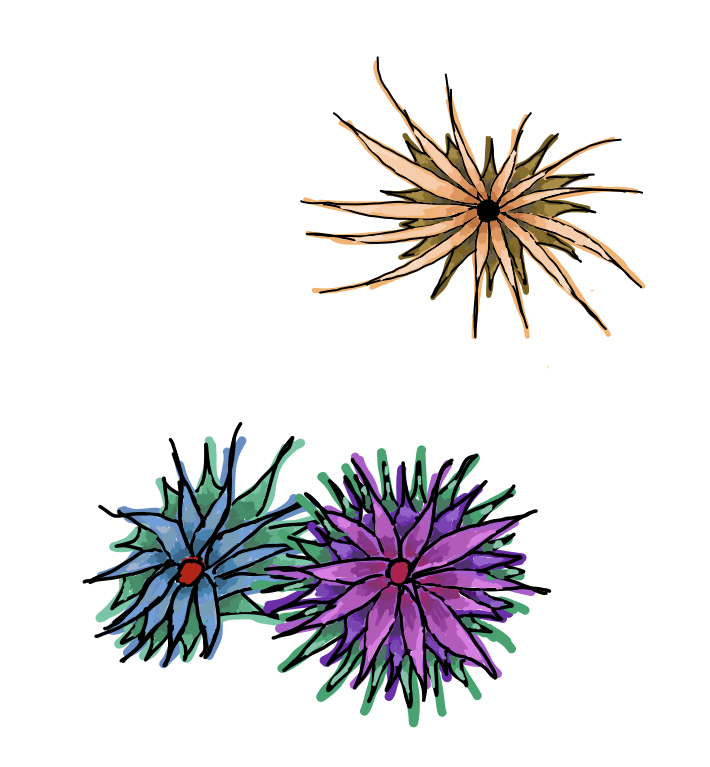
\includegraphics[scale=0.25]{floresportada.png}
}


\author{\LARGE Alonso Oma Alonso  \\ \LARGE Julia Pereda Vivo} % Your name

  
 
\date{\normalsize\today} % Today's date (\today) or a custom date



\begin{document}

\begin{titlepage}
	\maketitle
\end{titlepage}

\newpage
\tableofcontents
\newpage

\begin{section}{Tema 1:}

\end{section}

\newpage
\begin{section}{Tema 2: Movimiento}
    
    \begin{subsection}{Desplazamiento}
        \[\Delta \vec{r} = \vec{r'}-\vec{r} = (x'-x)\vec{u_x}+(y'-y)\vec{u_y}+(z'-z)\vec{u_z}=\Delta _x\vec{u_x}+\Delta _y\vec{u_y}+\Delta _z\vec{u_z}\]
    \end{subsection}

    \begin{subsection}{Velocidad promedio}
        \[\{\vec{v}\} = \frac{\Delta \vec{r}}{\Delta t} = \frac{\Delta x}{\Delta t}\vec{u_x}+\frac{\Delta y}{\Delta y}\vec{u_y}+\frac{\Delta z}{\Delta t}\vec{u_z}\]
    \end{subsection}

    \begin{subsection}{Velocidad instantánea}
        $\vec{v} = (v_x, v_y, v_z)$ vector en componentes cartesianas.  
                \[\vec{v} = \lim_{\Delta t \to 0} \vec{v} = \lim_{\Delta t \to 0} \frac{\Delta x}{\Delta t} \Rightarrow \vec{v} = \frac{d \vec{r}}{dt}\]
                Definiremos la 'celeridad' como el \textbf{módulo} $\vec{v}$.
                Por tanto, los cambios en la velocidad pueden deberse a dos factores: cambios en su módulo y cambios en su dirección.

                En una \negrita{trayectoria curvilínea} la direccció de la velocidad cambia debido a que $\vec{v}$ es tangente a la trayectoria y esta cambia constantemente. Por tanto, podemos concluir que cualquier objecto 
                que experimente una trayectoria curvilínea experimentará siempre una aceleración.

                Ahora, si conocemos la función que establece la velocidad de un objeto a través del tiempo $\left(\vec{v}_{instant} = f(t)\right)$ podemos hallar la función de desplazamiento del objeto:
                \[\integral{x_0}{t} dx = \integral{t_0}{t}v\cdot dt \Longrightarrow x = x_0 + \integral{t_0}{t} v \cdot dt\]
                Recordemos que $\integral{x_0}{x}dx = x-x_0$.
    \end{subsection}

    \begin{subsection}{Aceleración}
        \negrita{-Media:} 
                    \[<\vec{a}> = \frac{\Delta \vec{v}}{\Delta t} = \frac{\Delta v_x}{\Delta t}\vec{u_x}+\frac{\Delta v_y}{\Delta y}\vec{u_y}+\frac{\Delta v_z}{\Delta t}\vec{u_z}\]

                \negrita{-Instantánea:} $\vec{a} = \left(a_x, a_y, a_z\right)$ vector en componentes cartesianas.
                    \[\vec{a} = \limite{\Delta t}{0} \frac{\Delta \vec{v}}{\Delta t} \Rightarrow \vec{a} =  \frac{dv}{dt} = \frac{d}{dt}\left(\frac{dx}{dt}\right) \Rightarrow \vec{a} = \frac{d^2 x}{dt^2}\]

                Conocida la aceleración a traveás del tiempo, podemos obtener la ecuación de la velocidad:
                    \[ \{dv = \vec{a} dt \text{ y } \integral{v_0}{v}dv = v-v_0 \} \Longrightarrow \integral{v_0}{v} dv = \integral{t_0}{t} \vec{a} dt \Rightarrow v(t) = v_0 + \integral{t_0}{t} \vec{a}dt \]

                Nota: La aceleración 'direccional' apunta siempre hacia el lado cóncavo (zona del centro de la curvatura)
    \end{subsection}

    \begin{subsection}{Ecuaciones del movimiento}
        \begin{itemize}
            \item Conocida la posición en el tiempo:
                \[\begin{pmatrix}
                    x=x(t)\\
                    y = y(t)\\
                    z = z(t)
                \end{pmatrix} 
                \xRightarrow[]{derivar}
                \begin{pmatrix}
                    v_x(t) = \frac{dx(t)}{dt}\\
                    v_y(t) =\frac{dy(t)}{dt}\\
                    z_z(t) = \frac{dz(t)}{dt}
                \end{pmatrix}
                \xRightarrow[]{derivar}
                \begin{pmatrix}
                    a_x(t) = \frac{d^2 x(t)}{dt}\\
                    a_y(t) = \frac{d^2y(t)}{dt}\\
                    a_z(t) = \frac{d^2z(t)}{dt}
                \end{pmatrix}\]

            \item Conocida la $\vec{a}$:
                \[\begin{matrix}
                \vec{a} = \frac{d\vec{a}}{dt} \Longrightarrow \integral{\vec{v_0}}{\vec{v}} d\vec{v} = \integral{t_0}{t}\vec{a}(t')dt' \xRightarrow{integrar} \vec{v}(t) = \vec{v_0} + \integral{t_0}{t}\vec{a}(t')dt'\\
                \vec{v} = \frac{d\vec{r}}{dt} \xRightarrow{integrar} \integral{r_0}{r}d\vec{r} = \integral{t_0}{t}\vec{v}(t)\cdot dt \Longrightarrow\vec{r}(t) = \vec{r_0} + \integral{t_0}{t}\vec{v}(t')dt'
                \end{matrix}
                \Bigg\vert \Rightarrow\]
                \[\vec{r}(t)= \vec{r_0} + \integral{t_0}{t}\vec{v}(t')dt'\]

        \end{itemize}
    \end{subsection}

    \begin{subsection}{Particularizaciones:}
            \negrita{$\vec{a} = $ constante} (en módulo y dirección):
            \[\vec{v} = \vec{v_0} + \integral{t_0}{t}\vec{a}\cdot dt \xRightarrow[]{a=cte}\vec{v} = \vec{v_0} + \vec{a}(t-t_0)\]
            \[\vec{r}=\vec{r_0}   + \integral{t_0}{t}[\vec{v_0}+\vec{a}(t-t_0)]\cdot dt \Rightarrow \vec{r} = \vec{r_0} + \vec{v_0}(t-t_0) + \frac{1}{2}\vec{a}(t-t_0)^2 \longrightarrow\]
            \[\text{ecuación vectorial del plano: } (x, y, z) = (x_0, y_0, z_0) + \lambda(u_1, u_2, u_3) + \mu (v_1, v_2, v_3)\] 
            * En general $\vec{v_0}$ y $\vec{a}$ tienen direcciones diferentes.
            \[\integral{t_0}{t}\vec{v_0}\cdot dt + \vec{a}\integral{t_0}{t}(t-t_0  ) \cdot dt = \vec{v_0}(t-t_0  + \vec{a}\cdot \frac{(t-t_0)^2}{2})\]
            El extremo de $\vec{r}$ (trayectoria vista desde 0) se encuentra en el plano definido por $\vec{v_0}$, $\vec{a}$ que pasa por $\vec{r_0}$.

            Todo esto nos lleva a la conslusión de que si $\vec{a} = $ cte el movimiento se realiza en un plano
    \end{subsection}

    \begin{subsection}{Tiro parabólico}
        \begin{tikzpicture}
            \begin{axis} [axis lines=center]
                \addplot [domain = 0:10, smooth, thick] {((-1)/5)*x^2 + 2*x};
            \end{axis}
            \node at (3.5, 6) {$\varphi (t)$};
            \draw[-stealth] (3.5,3) -- (3.5,2);
            \node at (3.5, 1.75) {$\vec{a} = \vec{g}$};
        \end{tikzpicture}

        En el tiro parabólico se tiene que $\vec{a} = \vec{g}$.
    \end{subsection}

\end{section}

\end{document}